\section{The Differential Horizon of Intelligence}

\subsection{Overview}

\S{}7 showed the dynamical consequence of accumulated correctness: branching explosion. \S{}8 showed the structural fact behind it: no stopping operator exists inside individual inference. This section turns that negative result around. It asks what must be externalized if individual intelligence cannot close on itself.

The answer is a local horizon-form. The individual inferential system reaches a descriptive boundary: it requires stopping, persistence, and revisability, but cannot generate the stopping operator internally.

\subsection{The structural necessity of crossing}

Let \(\mathcal{R}\) be the structure of individual causal inference. \S{}8 stated:
\[
\mathcal{T}\notin \mathrm{Internal}(\mathcal{R}).
\]
If stopping is required but not generated internally, then stopping must be stabilized through an externalized structure:
\[
\mathcal{T}\in \mathrm{External}(\mathcal{R}).
\]

Here \(\mathrm{External}\) does not mean a spatial outside or hidden region. It means records, responses, agreements, delays, and distributed responsibility: structures that reorganize the observational window of inference.

This reorganization is called crossing. Crossing is not a heroic leap beyond a boundary. It is the structural transition from individual inference to externalized stopping.

\subsection{What is externalized}

Four functions are externalized.

\textbf{Stopping judgments.}
The judgment that a line of inference is complete is stabilized by response, agreement, institutional decision, or other externalized structure.

\textbf{Records.}
Inference is fixed as log, text, data, or trace. A log is not merely memory. It preserves inference outside the immediate temporal flow of the individual system.

\textbf{Temporal delay.}
Delay interrupts runaway inference and makes revision possible. Waiting for response, documentation, review, or deliberation imposes time from outside the individual loop.

\textbf{Distribution of responsibility.}
Because stopping is externally stabilized, responsibility cannot be monopolized by the individual system. It becomes distributed across agents, records, procedures, and contexts.

None of these guarantees correctness. Externalization guarantees only a more limited and more important property: inference can stop, persist, and later be revised.

\subsection{Naming the boundary}

The boundary at which individual inference cannot complete its own stopping is named:

\begin{quote}
\textbf{the differential horizon of intelligence}.
\end{quote}

This naming connects the present paper to VED Vol.4 \citep{VEDVol4}. In Vol.4, the \DH{} is not a wall located somewhere in spacetime. It is the descriptive boundary that appears when a generated description attempts to convert the absence of difference into an ordinary describable state.

At the intelligence layer, the same structural form appears locally. Individual inference cannot internally generate the externalized stopping structures it requires. When pushed toward that limit, it produces branching explosion rather than closure. Contact with the boundary is absorbed as finite internal representation: log, response, agreement, delay.

Thus the \DHI{} is not a separate absolute horizon. It is the \DH{} appearing as a local horizon-form inside the observational window of intelligence.

\begin{figure}[H]
\centering
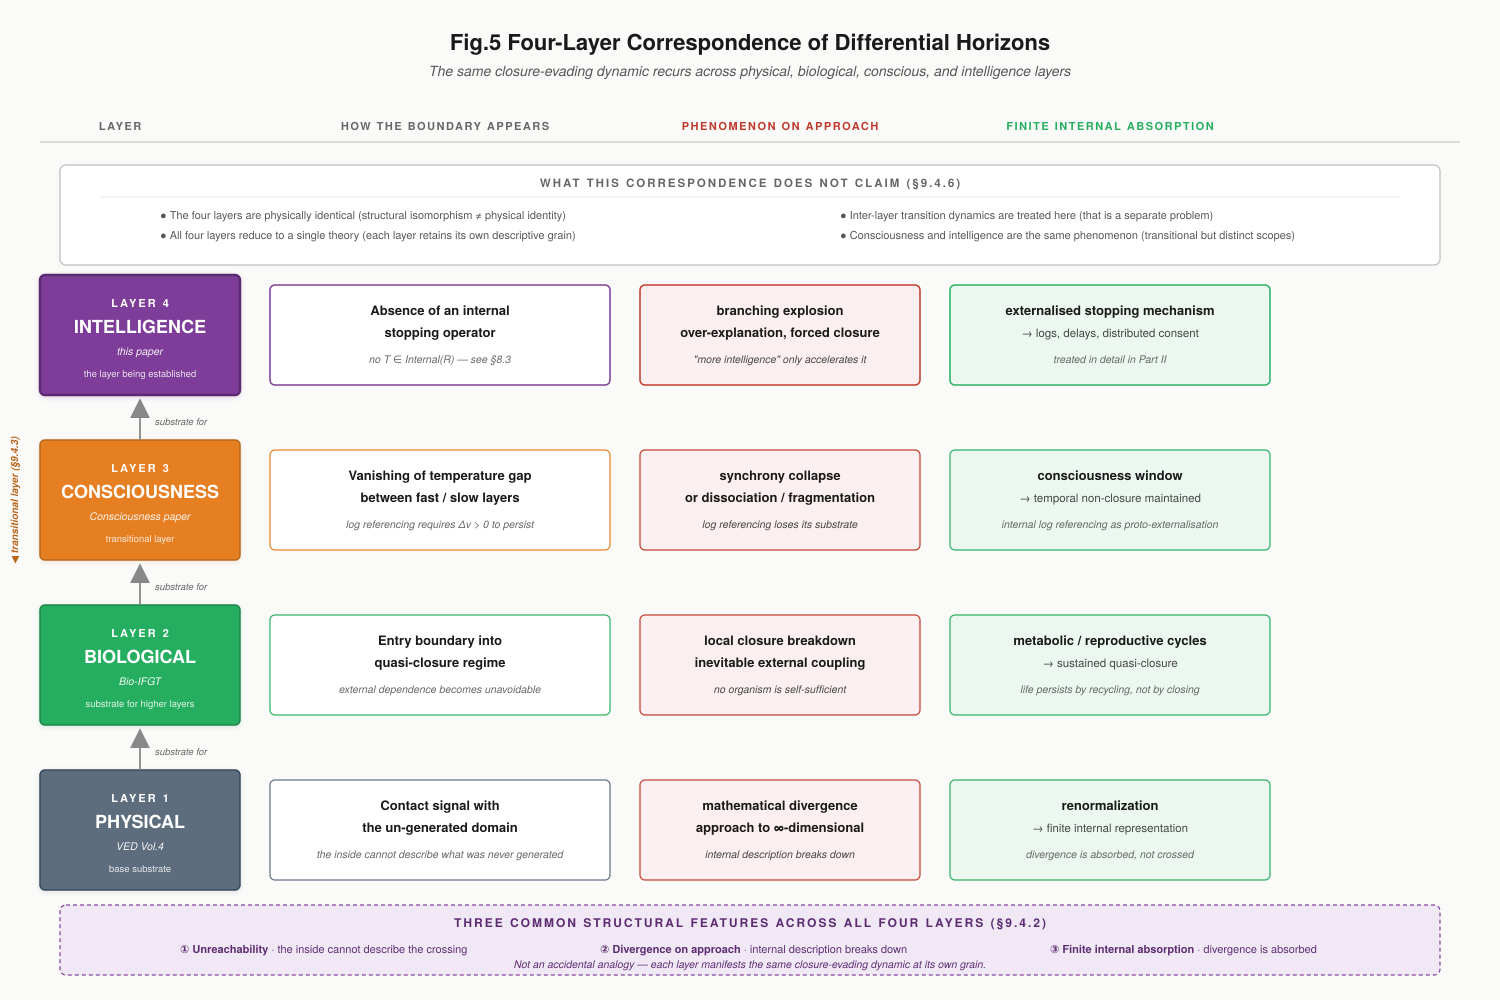
\includegraphics[width=\textwidth]{figures/fig5_four_layer_correspondence.png}
\caption{Four-layer correspondence of Differential Horizon forms. The same closure-evading dynamic recurs across physical, biological, consciousness, and intelligence layers without implying physical identity among the layers.}
\label{fig:intelligence_part1_5}
\end{figure}

\subsection{Layered correspondence}

The four relevant layers are:

\begin{table}[H]
\centering
\small
\begin{tabularx}{\textwidth}{>{\raggedright\arraybackslash}X>{\raggedright\arraybackslash}X>{\raggedright\arraybackslash}X>{\raggedright\arraybackslash}X}
\toprule
Layer & Boundary form & Phenomenon on approach & Finite absorption \\
\midrule
Physical (VED Vol.4) & descriptive boundary where absence of difference cannot become an ordinary state & divergence, asymptotic expansion & renormalization \\
Biological (Bio-IFGT) & entry boundary into quasi-closure & local closure breakdown, unavoidable external dependence & metabolic and reproductive cycles \\
Consciousness & loss of fast/slow temperature gap & synchrony collapse or dissociation & consciousness window and log referencing \\
Intelligence & absence of an internal stopping operator & over-explanation, forced closure, branching explosion & externalized stopping mechanisms \\
\bottomrule
\end{tabularx}
\end{table}

These layers are not physically identical. They do not reduce to a single theory, and their transition dynamics are not treated here. The correspondence is structural: each layer exhibits non-closure, divergence on approach, and finite internal absorption.

\subsection{Connection to subsequent work}

This paper names the local horizon-form and derives the need for crossing. It does not describe the detailed social or institutional mechanisms that operate after crossing. Those belong to Intelligence Part II.

Part II will treat externalized stopping mechanisms, log-based persistence, distributed revisability, collective decision-making, and institutional forms. The present paper supplies the structural constraint that makes those topics necessary.

\subsection{Summary}

\begin{quote}
The differential horizon of intelligence is the local form of the \DH{} that appears when individual inference requires stopping but cannot generate its own stopping operator.
\end{quote}

\begin{quote}
Crossing this horizon does not guarantee correctness. It permits inference to stop, persist, and be revised.
\end{quote}
